\documentclass[letterpaper,12pt]{article}

\usepackage[margin=1in]{geometry}
\usepackage{titling}
\usepackage{graphicx}

\setlength{\droptitle}{-0.75in}
\setlength{\parindent}{0in}
\setlength{\parskip}{\baselineskip}

\title{Fault Tolerance in Block-Level Caching}
\author{
  Jesus Ramos \\ \texttt{jramo028@fiu.edu} \and
  Douglas Otstott \\ \texttt{dotst001@fiu.edu}
}
\date{}

\begin{document}

\maketitle

\section*{Problem Statement}

Many companies are switching to warehouse scale computing to deal with
increasing computing demands due to the cost and efficiency of
warehouse architecture. Rather than trying to prevent failure, most
warehouse scale computing solutions accept failure and attempt to
integrate recovery as seamlessly as possible.

Dependability and reliability are two important factors when dealing
with cloud and warehouse scale computing. Systems should be robust and
be able to recover from errors and failure effectively and quickly.

Fault tolerance is still a major issue in cloud based systems that
employ caching. Currently in the event of an error or power failure
all data that was pending to be written back is lost along with
currently cached data. In some cases minor data loss is acceptable,
but in most cases even minor loss of data can result in larger
problems and error recovery can become very complex depending on the
type and quantity of data lost.

% end section Problem Statement

\section*{Problem Background}

\begin{center}
  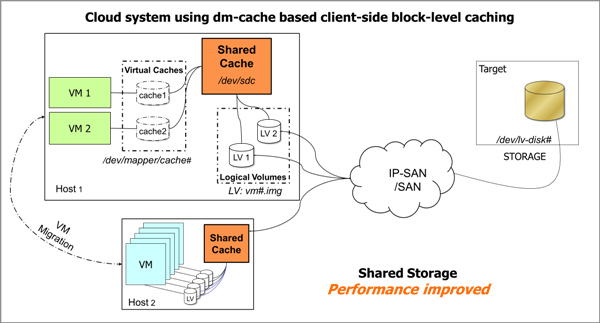
\includegraphics{../Images/NewerImage.png}
\end{center}

Many large scale cloud based systems employ network storage due to the
physical limitations of local storage devices. Basically, each host
machine in the cloud is connected to a small number of machines which
are responsible for all persistent data management across the system.
These machines create what is known as a Storage Area Network (SAN).
SAN's are a common solution used by cloud service providers due to the
simplification of virtual machine migration and increased data
reliability \cite{Datacenter}. While this solves the storage size
problem it also increases the response latency and creates a bandwidth
issue due to the sheer volume of requests constantly sent to the
storage devices.

Local caches are employed by many systems as a means to bring in the
most frequently used data to more local storage devices to reduce
latency and alleviate pressure on the main storage system. DM-Cache is
an open-source block-level caching solution developed as a Linux
kernel module. DM-Cache allows host machines to store the most
recently used blocks in a designated storage device. Preliminary
testing on DM-Cache indicates a significant improvement in systems
where numerous hosts and virtual machines create a bottleneck in terms
of network storage bandwidth. However, local caching introduces a new
problem in terms of fault tolerance as locally modified blocks are
lost in the event of system failure.

% end section Problem Background

\section*{Proposed Solution}

The solution to the inherent fault intolerance of local caching is to
move the metadata from non-persistent memory to the persistent cache
device. In this way, we can reconstruct the state of the cache in the
event of power loss or system failure to within some margin of
error. To minimize the performance overhead this policy would
necessitate, we also propose that recently used metadata should be
cached in memory and changes to metadata should be written back to
disk asynchronously. This of course would prevent very recent changes
to metadata from being recovered if they had yet not been committed to
disk. However, we believe this is a fair trade off in terms of fault
tolerance versus performance.

DM-Cache currently has two variations of organizing metadata in its
implementation. One uses a hash table for a metadata structure and the
other uses a radix tree. Currently, the plan is to attempt
implementation on both concurrently and focus on the either solution
in the interest of time. The radix tree implementation still has some
bugs that still need to be addressed. Depending on the complexity of
solving these issues, we may focus on the hash table implementation in
order to accommodate the projects time constraints.

% end section Proposed Solution

\pagebreak
\section*{Project Timeline}

\begin{description}
  \item[February 26th] - Begin Preliminary Testing (Radix Tree)
  \item[March 1st] - Begin solution implementation (Radix Tree / Hash
  Table)
  \item[April 5th] - Debug solution (Hash Table)
  \item[April 10th] - Begin Evaluation
  \item[April 15th] - Conclude Evaluation
  \item[April 20th] - Write a paper and presentation
\end{description}

% end section Project Timeline

\section*{Project Evaluation}

In this project we will evaluate the overhead introduced in DM-Cache
by persisting metadata to the disk. The first round of testing will
involve running I/O benchmarks with and without metadata persistence
and compare the results to determine the performance decrease created
by the extra overhead. The second test will evaluate the actual
effectiveness of the data recovery mechanism. The plan is to execute a
standardize workload (such a kernel compilation) using a cache, and we
shall unplug the machine as the execution concludes. We shall then
measure the degree which data can be recovered in the metadata
persistent cache compared to the original implementation of DM-Cache.

% end section Project Evaluation

\section*{Related Work}

Error recovery in storage systems that employ caching techniques is
not a new idea and has been shown to work quickly and reliably in DRAM
based systems \cite{RAMCloud}.

Recovery of persisted data in the event of a system failure using a
transactional approach can ensure correctness in persisted data as
well as provide mechanisms for error recovery \cite{NVHeaps}.

Storage class memory devices have been used to create persistent
memory models allowing for in memory structures to be persisted
quickly and reliably \cite{Mnemosyne}. This idea can be extended to
solid state drives whose performance is very close to that of storage
class memory devices.

Transactional operations for fault tolerant systems has been suggested
before and was shown to be tunable to provide as much performance or
overhead that the programmer wanted \cite{FaulTM}.

Different communication architectures exist for handling network
bandwidth issues based on using hierarchies of commodity switches but
these solutions can incur high cost \cite{Network}. With this proposal
we seek to try and alleviate more of the network pressure to reduce
costs of such solutions.

The case for using SSD's in an enterprise database setting was
suggested by Lee et al.\ where they were able to show that SSD's could
improve throughput of enterprise database applications
\cite{EnterpriseSSD}. This study also reported that there was room
left for write optimization on SSD's which could allow for even higher
performance gains.

Efficient data structures for SSD's have been proposed in the past. Wu
et al.\ proposed a B-tree structure for use within the SSD's FTL (Flash
Translation Layer) which lead to better random right throughput, lower
energy consumption, and less write-wearing \cite{FlashB-Tree}. Li et
al.\ proposed another tree-like structure called an FD-Tree which led
to similar results \cite{FD-Tree}.

% end section Related Work

\bibliography{proposal}
\bibliographystyle{acm}

\end{document}
